%% figs/failure_bucket_breakdown.tex — TikZ wireframe stub for §6 visual.
%% Per-LLM stacked-bar failure-bucket breakdown.
%% Populate from paper/data/extracted_failures.csv after mlcad_runner D8.
%%
%% NB: §6 currently uses Table 4 as the primary failure-bucket
%% deliverable; this figure is an optional visual companion if page
%% budget allows. Wireframe only.

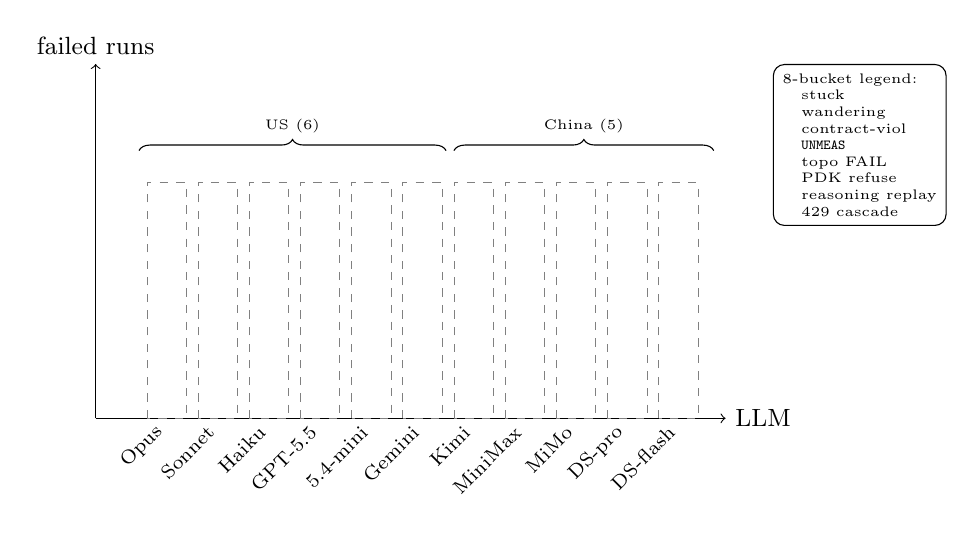
\begin{tikzpicture}
  %% Axes
  \draw[->] (0,0) -- (8.0,0) node[right] {\small LLM};
  \draw[->] (0,0) -- (0,4.5) node[above] {\small failed runs};

  %% 11 stacked-bar wireframe slots (one per LLM, dashed outline only)
  \foreach \i in {1,...,11} {%
    \draw[dashed, gray, very thin]
      ({\i*0.65},0) rectangle ({\i*0.65+0.5},3.0);
  }

  %% Vendor-cohort grouping brackets (US block / China block)
  \draw[decorate, decoration={brace, amplitude=4pt}]
    (0.55,3.4) -- (4.45,3.4)
    node[midway, above=3pt, font=\tiny] {US (6)};
  \draw[decorate, decoration={brace, amplitude=4pt}]
    (4.55,3.4) -- (7.85,3.4)
    node[midway, above=3pt, font=\tiny] {China (5)};

  %% LLM tick labels
  \foreach \i/\lbl in {%
    1/Opus, 2/Sonnet, 3/Haiku,
    4/{GPT-5.5}, 5/{5.4-mini}, 6/Gemini,
    7/Kimi, 8/MiniMax, 9/MiMo,
    10/{DS-pro}, 11/{DS-flash}} {%
    \node[rotate=45, anchor=east, font=\scriptsize]
      at ({\i*0.65+0.25},-0.05) {\lbl};
  }

  %% Bucket legend (right of bars)
  \node[draw, rounded corners, font=\tiny, align=left,
        anchor=north west] at (8.6,4.5) {%
    8-bucket legend: \\
    \quad stuck \\
    \quad wandering \\
    \quad contract-viol \\
    \quad \texttt{UNMEAS} \\
    \quad topo FAIL \\
    \quad PDK refuse \\
    \quad reasoning replay \\
    \quad 429 cascade};
\end{tikzpicture}
